\documentclass{article}
\usepackage{fancyhdr}
\usepackage{tikz}
\usepackage{xcolor}
\usepackage{pgfplots}
\usepackage{pst-func}

\usetikzlibrary{trees}

\pagestyle{fancy}
\setlength{\headheight}{35pt}
\lhead{Datenstrukturen \& Algorithmen\\Sommersemester2020\\Übungsblatt 4}
\chead{}
% bfseries
\rhead{Ciheng Zhang(3472321)\\Yao He(3487882)\\YuchanBian(3496226)}
\cfoot{\thepage}
\renewcommand{\headrulewidth}{0.4pt}

\begin{document}
\begin{titlepage}
    \title{\Huge \textbf{Datenstrukturen \& Algorithmen Gruppeübung\\Gruppe 10} }
    \author{\LARGE \textsl{Ciheng Zhang (3472321) zch3183505@gmail.com}\\\LARGE \textsl{Yao He (3487882) st168323@stud.uni-stuttgart.de}\\\LARGE \textsl{Yuchan Bian (3496226) st170182@stud.uni-stuttgart.de} \\[200pt]}
    \date{\today}
    \maketitle
    \thispagestyle{empty}
\end{titlepage}
\newpage
\section{Aufgabe 1}
\subsection*{a.}
% 树结构
\begin{tikzpicture}[sibling distance=10em,
  every node/.style = {shape=rectangle, rounded corners,
    draw, align=center,
    top color=white, bottom color=blue!20}]]
  \node {41 69}
    child { node {23}
            child{node{18 22}} 
            child{node[xshift=-5em]{28 33 40}}}
    child { node {46 50}
            child{node[xshift=5em]{42}} 
            child{node{47}}
            child{node[xshift=-5em]{60 62 63}}}
    child { node {71}
            child{node[xshift=5em]{70}} 
            child{node[xshift=-1em]{73 88 94}}};
\end{tikzpicture}
\\Nach 36 gefügt:\\
% 树结构
\begin{tikzpicture}[sibling distance=8.5em,
    every node/.style = {shape=rectangle, rounded corners,
      draw, align=center,
      top color=white, bottom color=blue!20}]]
    \node {41 69}
      child { node {23 33}
              child{node{18 22}}
              child{node[xshift=-5em]{28}} 
              child{node[xshift=-9em]{36 40}}}
      child { node {46 50}
              child{node[xshift=5em]{42}} 
              child{node{47}}
              child{node[xshift=-5em]{60 62 63}}}
      child { node {71}
              child{node[xshift=5em]{70}} 
              child{node{73 88 94}}};
  \end{tikzpicture}
  \\Nach 92 gefügt:\\
  % 树结构
\begin{tikzpicture}[sibling distance=8em,
    every node/.style = {shape=rectangle, rounded corners,
      draw, align=center,
      top color=white, bottom color=blue!20}]]
    \node {41 69}
        child { node {23 33}
                child{node{18 22}}
                child{node[xshift=-5em]{28}} 
                child{node[xshift=-9em]{36 40}}}
      child { node {46 50}
              child{node[xshift=5em]{42}} 
              child{node{47}}
              child{node[xshift=-4em]{60 62 63}}}
      child { node {71 88}
              child{node[xshift=7em]{70}}
              child{node[xshift=2em]{73}} 
              child{node[xshift=-1em]{92 94}}};
  \end{tikzpicture}
  \\Zuerst sucht man die Baum. Dann man soll 36 in Knote 28,33,40 einfügen. Aber diese Knote ist ein 4Knote. Sollt man diese Knote
  aufteilrn. 33 nach oben ziehen und 40 nach recht ziehen.Dann 36 einfügen. Dann man soll die Zahl 92 einfügen. gleich wie 36 gemacht
  .Zerst man split die Knote 73,88,94.Dann 92 einfügen.\\
 
  \subsection*{b.}
  % 红黑树结构
  \begin{tikzpicture}[sibling distance=10em,
    black/.style = {shape=rectangle, rounded corners,
      draw, align=center,
      color=black},
    red/.style = {shape=rectangle, rounded corners,
      draw, align=center,
     color=red}] 
      ]
    \node[black]{69}
        child{node[red]{41}
                child{node[black]{33}
                        child{node[red]{23}
                                child{node[black]{22}
                                        child{node[red]{18}}}
                                child{node[black,xshift=-3em]{28}}}
                        child{node[black,xshift=-3em]{40}
                                child{node[red,xshift=-3em]{36}}}}
                child{node[black]{50}
                        child{node[red]{46}
                                child{node[black,xshift=2em]{42}}
                                child{node[black,xshift=-2em]{47}}}
                        child{node[black,xshift=-2em]{62}
                                child{node[red,xshift=2em]{60}}
                                child{node[red,xshift=-3em]{63}}}}}
        child{node[black,xshift=4em]{88}
                child{node[red,xshift=4em]{71}
                        child{node[black,xshift=4em]{70}}
                        child{node[black,xshift=-1em]{73}}}
                child{node[black]{94}
                        child{node[red]{92}}}};
  \end{tikzpicture}
  \subsection*{c.}

   % 红黑树结构
   \begin{tikzpicture}[sibling distance=10em,
    black/.style = {shape=rectangle, rounded corners,
      draw, align=center,
      color=black},
    red/.style = {shape=rectangle, rounded corners,
      draw, align=center,
     color=red}] 
      ]
    \node[black]{69}
        child{node[red]{41}
                child{node[black]{33}
                        child{node[red]{23}
                                child{node[black]{22}
                                        child{node[red]{18}}}
                                child{node[black,xshift=-3em]{28}}}
                        child{node[black,xshift=-3em]{40}
                                child{node[red,xshift=-3em]{36}}}}
                child{node[black]{50}
                        child{node[red]{46}
                                child{node[black,xshift=2em]{42}}
                                child{node[black,xshift=-2em]{47}}}
                        child{node[black,xshift=-2em]{62}
                                child{node[red,xshift=2em]{60}
                                        child{node[red,xshift=-2em]{51}}}
                                child{node[red,xshift=-3em]{63}}}}}
                                child{node[black,xshift=4em]{88}
                                child{node[red,xshift=4em]{71}
                                        child{node[black,xshift=4em]{70}}
                                        child{node[black,xshift=-1em]{73}}}
                                child{node[black]{94}
                                        child{node[red]{92}}}};
  \end{tikzpicture}
  \\Zuerst sucht man die richtige Position, die die Zahl 51 einfügen soll.\\
    % 红黑树结构
    \begin{tikzpicture}[sibling distance=10em,
        black/.style = {shape=rectangle, rounded corners,
          draw, align=center,
          color=black},
        red/.style = {shape=rectangle, rounded corners,
          draw, align=center,
         color=red}] 
          ]
        \node[black]{69}
            child{node[red]{41}
                    child{node[black]{33}
                            child{node[red]{23}
                                    child{node[black]{22}
                                            child{node[red]{18}}}
                                    child{node[black,xshift=-3em]{28}}}
                            child{node[black,xshift=-3em]{40}
                                    child{node[red,xshift=-3em]{36}}}}
                    child{node[black]{50}
                            child{node[red]{46}
                                    child{node[black,xshift=2em]{42}}
                                    child{node[black,xshift=-2em]{47}}}
                            child{node[red,xshift=-2em]{62}
                                    child{node[black,xshift=2em]{60}
                                            child{node[red,xshift=-2em]{51}}}
                                    child{node[black,xshift=-3em]{63}}}}}
                                    child{node[black,xshift=4em]{88}
                                    child{node[red,xshift=4em]{71}
                                            child{node[black,xshift=4em]{70}}
                                            child{node[black,xshift=-1em]{73}}}
                                    child{node[black]{94}
                                            child{node[red]{92}}}};
      \end{tikzpicture}
      \\Denn die Parent node und die UncleNode sind rot. Dann farbt man die ParntNode und UncleNode schwarz und GrandNode rot. Dann node gleich wie GrandNode.
\section{Aufgabe 2}
Lösung im beigefügten Eclipse-Project
\section{Aufgabe 3}
Lösung im beigefügten Eclipse-Project
\newpage
\section{Aufgabe 4}
Zuerst die erst 4 Zähle einfügen.\\
\begin{tikzpicture}[sibling distance=8em,
    every node/.style = {shape=rectangle, rounded corners,
      draw, align=center,
      top color=white, bottom color=blue!20}]]
    \node {22 26 61 71};
  \end{tikzpicture}\\
  Dann die 5 Element einfügen,und split.\\
  \begin{tikzpicture}[sibling distance=8em,
    every node/.style = {shape=rectangle, rounded corners,
      draw, align=center,
      top color=white, bottom color=blue!20}]]
    \node {22 26 61 61 71};
  \end{tikzpicture}
  \begin{tikzpicture}[sibling distance=8em,
    every node/.style = {shape=rectangle, rounded corners,
      draw, align=center,
      top color=white, bottom color=blue!20}]]
    \node {61}
        child{node{22 26}}
        child{node{61 71}};
  \end{tikzpicture}
  \\Dann die weitere Element einfügen:\\
  \begin{tikzpicture}[sibling distance=8em,
    every node/.style = {shape=rectangle, rounded corners,
      draw, align=center,
      top color=white, bottom color=blue!20}]]
    \node {61}
        child{node{22 26}}
        child{node{61 67 71}};
  \end{tikzpicture}
  \begin{tikzpicture}[sibling distance=8em,
    every node/.style = {shape=rectangle, rounded corners,
      draw, align=center,
      top color=white, bottom color=blue!20}]]
    \node {61}
        child{node{22 26}}
        child{node{61 67 70 71}};
  \end{tikzpicture}
  \begin{tikzpicture}[sibling distance=8em,
    every node/.style = {shape=rectangle, rounded corners,
      draw, align=center,
      top color=white, bottom color=blue!20}]]
    \node {61}
        child{node{22 26 33}}
        child{node{61 67 70 71}};
  \end{tikzpicture}
  \begin{tikzpicture}[sibling distance=8em,
    every node/.style = {shape=rectangle, rounded corners,
      draw, align=center,
      top color=white, bottom color=blue!20}]]
    \node {61}
        child{node{22 26 33 40}}
        child{node{61 67 70 71}};
  \end{tikzpicture}
  \begin{tikzpicture}[sibling distance=8em,
    every node/.style = {shape=rectangle, rounded corners,
      draw, align=center,
      top color=white, bottom color=blue!20}]]
    \node {61}
        child{node{22 26 33 40 52}}
        child{node{61 67 70 71}};
  \end{tikzpicture}\\
  Dann noch mal split:\\
  \begin{tikzpicture}[sibling distance=8em,
    every node/.style = {shape=rectangle, rounded corners,
      draw, align=center,
      top color=white, bottom color=blue!20}]]
    \node {33 61}
        child{node{22 26}}
        child{node{40 52}}
        child{node{61 67 70 71}};
  \end{tikzpicture}
  \\Dann weitere einfügen:\\
  \begin{tikzpicture}[sibling distance=8em,
    every node/.style = {shape=rectangle, rounded corners,
      draw, align=center,
      top color=white, bottom color=blue!20}]]
    \node {33 61}
        child{node{22 26}}
        child{node{36 40 52}}
        child{node{61 67 70 71}};
  \end{tikzpicture}
  \begin{tikzpicture}[sibling distance=8em,
    every node/.style = {shape=rectangle, rounded corners,
      draw, align=center,
      top color=white, bottom color=blue!20}]]
    \node {33 61}
        child{node{22 26}}
        child{node{36 40 43 52}}
        child{node{61 67 70 71}};
  \end{tikzpicture}
  \begin{tikzpicture}[sibling distance=8em,
    every node/.style = {shape=rectangle, rounded corners,
      draw, align=center,
      top color=white, bottom color=blue!20}]]
    \node {33 61}
        child{node{22 26}}
        child{node{36 40 43 51 52}}
        child{node{61 67 70 71}};
  \end{tikzpicture}
  \\noch mal split:\\
  
\begin{tikzpicture}[sibling distance=8em,
    every node/.style = {shape=rectangle, rounded corners,
      draw, align=center,
      top color=white, bottom color=blue!20}]]
    \node {33 43 61}
        child{node{22 26}}
        child{node{36 40}}
        child{node{51 52}}
        child{node{61 67 70 71}};
  \end{tikzpicture}\\
  weitere einfügen:\\
  
\begin{tikzpicture}[sibling distance=8em,
    every node/.style = {shape=rectangle, rounded corners,
      draw, align=center,
      top color=white, bottom color=blue!20}]]
    \node {33 43 61}
        child{node{22 26}}
        child{node{36 40}}
        child{node{51 52}}
        child{node{61 67 70 71 72}};
  \end{tikzpicture}\\
  split:\\
  
\begin{tikzpicture}[sibling distance=8em,
    every node/.style = {shape=rectangle, rounded corners,
      draw, align=center,
      top color=white, bottom color=blue!20}]]
    \node {33 43 61 70}
        child{node{22 26}}
        child{node{36 40}}
        child{node{51 52}}
        child{node{61 67}}
        child{node{71 72}};
  \end{tikzpicture}\\
  weiter:\\
  
\begin{tikzpicture}[sibling distance=8em,
    every node/.style = {shape=rectangle, rounded corners,
      draw, align=center,
      top color=white, bottom color=blue!20}]]
    \node {33 43 61 70}
        child{node{22 26}}
        child{node{36 40}}
        child{node{51 52}}
        child{node{61 67}}
        child{node{71 72 81}};
  \end{tikzpicture}\\
  
\begin{tikzpicture}[sibling distance=8em,
    every node/.style = {shape=rectangle, rounded corners,
      draw, align=center,
      top color=white, bottom color=blue!20}]]
    \node {33 43 61 70}
        child{node{22 26}}
        child{node{36 40}}
        child{node{51 52}}
        child{node{61 67}}
        child{node{71 72 81 83}};
  \end{tikzpicture}\\
  
\begin{tikzpicture}[sibling distance=8em,
    every node/.style = {shape=rectangle, rounded corners,
      draw, align=center,
      top color=white, bottom color=blue!20}]]
    \node {33 43 61 70}
        child{node{22 26}}
        child{node{36 40}}
        child{node{51 52}}
        child{node{61 67}}
        child{node{71 72 74 81 83}};
  \end{tikzpicture}\\
  split:
  \begin{tikzpicture}[sibling distance=8em,
    every node/.style = {shape=rectangle, rounded corners,
      draw, align=center,
      top color=white, bottom color=blue!20}]]
    \node {33 43 61 70}
        child{node{22 26}}
        child{node{36 40}}
        child{node{51 52}}
        child{node{61 67}}
        child{node[xshift=-3em]{74}
                child{node{71 72}}
                child{node[xshift=-2em]{81 83}}};
  \end{tikzpicture}\\

  
\begin{tikzpicture}[sibling distance=8em,
    every node/.style = {shape=rectangle, rounded corners,
      draw, align=center,
      top color=white, bottom color=blue!20}]]
    \node {33 43 61 70 74}
        child{node{22 26}}
        child{node{36 40}}
        child{node{51 52}}
        child{node{61 67}}
        child{node{71 72}}
        child{node{81 83}};
  \end{tikzpicture}\\

  \begin{tikzpicture}[sibling distance=8em,
    every node/.style = {shape=rectangle, rounded corners,
      draw, align=center,
      top color=white, bottom color=blue!20}]]
    \node {61}
        child{node{33 43}
                child{node{22 26}}
                child{node[xshift=-3em]{36 40}}
                child{node[xshift=-6em]{51 52}}}
        child{node{70 74}
                child{node[xshift=6em]{61 67}}
                child{node[xshift=3em]{71 72}}
                child{node[xshift=2em]{81 83}}};

  \end{tikzpicture}\\
\end{document}
